\part{Stacks and queues}
\frame{\partpage}

\begin{frame}{Stacks and queues}
	\begin{columns}
		\pause
		\begin{column}{0.3\textwidth}
			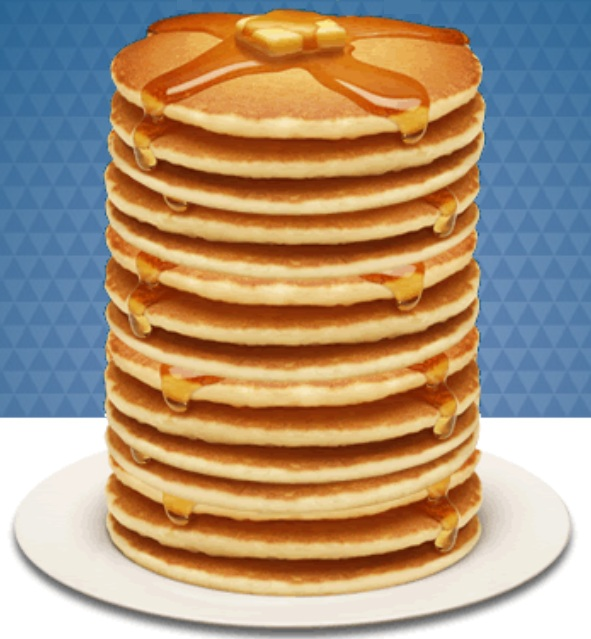
\includegraphics[width=\textwidth]{stack}
		\end{column}
		\begin{column}{0.68\textwidth}
			\begin{itemize}
				\item A \textbf{stack} is a \textbf{last-in first-out (LIFO)} data structure
				\pause\item Items can be \textbf{pushed} to the \textbf{top} of the stack
				\pause\item Items can be \textbf{popped} from the \textbf{top} of the stack
			\end{itemize}
		\end{column}
	\end{columns}
	\begin{columns}
		\pause
		\begin{column}{0.3\textwidth}
			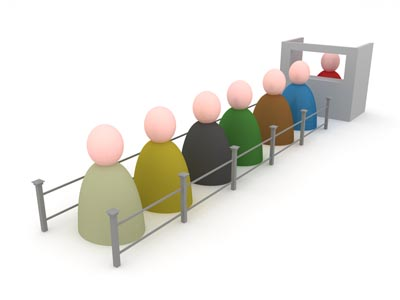
\includegraphics[width=\textwidth]{queue}
		\end{column}
		\begin{column}{0.68\textwidth}
			\begin{itemize}
				\item A \textbf{queue} is a \textbf{first-in first-out (FIFO)} data structure
				\pause\item Items can be \textbf{enqueued} to the \textbf{back} of the queue
				\pause\item Items can be \textbf{dequeued} from the \textbf{front} of the queue
			\end{itemize}
		\end{column}
	\end{columns}
\end{frame}

\begin{frame}{Lists in Python}
	\begin{itemize}
		\pause\item Implemented as a (variable-sized) \textbf{array}
		\pause\item Appending is $O(1)$
		\pause\item Inserting is $O(n)$
		\pause\item Deleting is $O(n)$
	\end{itemize}
\end{frame}

\begin{frame}{Stacks in Python}
	\begin{itemize}
		\pause\item Stacks can be implemented efficiently as lists
		\pause\item \lstinline{append} method adds an element to the end of the list
			\begin{itemize}
				\pause\item What is the time complexity?
			\end{itemize}
		\pause\item \lstinline{pop} method removes and returns the last element of the list
			\begin{itemize}
				\pause\item What is the time complexity?
			\end{itemize}
	\end{itemize}
\end{frame}

\begin{frame}{Queues in Python}
	\begin{itemize}
		\pause\item Queues can be implemented as lists, but not efficiently
		\pause\item Could use \lstinline{append(item)} to enqueue and \lstinline{pop(0)} to dequeue
			\begin{itemize}
				\pause\item What is the time complexity of \lstinline{pop(0)}?
			\end{itemize}
		\pause\item Could use \lstinline{insert(0, item)} to enqueue and \lstinline{pop()} to dequeue
			\begin{itemize}
				\pause\item What is the time complexity of \lstinline{insert(0, item)}?
			\end{itemize}
		\pause\item \lstinline{deque} (from the \lstinline{collections} module) implements an efficient
			\textbf{double-ended queue}
		\pause\item Provides methods \lstinline{append}, \lstinline{appendleft}, \lstinline{pop}, \lstinline{popleft}
			\begin{itemize}
				\pause\item All of which are $O(1)$
			\end{itemize}
	\end{itemize}
\end{frame}

\begin{frame}{Stacks and function calls}
	\begin{itemize}
		\pause\item Stacks are used to implement \textbf{nested function calls}
		\pause\item Each invocation of a function has a \textbf{stack frame}
		\pause\item This specifies information like \textbf{local variable values} and \textbf{return address}
		\pause\item Calling a function \textbf{pushes} a new frame onto the stack
		\pause\item Returning from a function \textbf{pops} the top frame off the stack
	\end{itemize}
\end{frame}
